% Part 2: how the country name reaches the decision. Include from country_effect/main.tex with
%   % Part 2: how the country name reaches the decision. Include from country_effect/main.tex with
%   % Part 2: how the country name reaches the decision. Include from country_effect/main.tex with
%   % Part 2: how the country name reaches the decision. Include from country_effect/main.tex with
%   \input{part2_attribution/report/part2_section}
% Numbers are taken from part2_attribution/report/facts.json and the stage results.json files.

\section{How the Country Reaches the Decision}
\label{sec:part2}

We trace how the country name's influence travels through Llama-3.2-3B-Instruct to the BV decision. We ask when the country becomes readable as an answer preference, where in layer and token position its influence is carried, and in what form it reaches the answer.

\subsection{Setup}

\paragraph{Notation.}
The model has $L=28$ blocks. $h_{\ell,t}$ is the residual stream after block $\ell$ at position $t$, and $T$ is the final prompt token (``\textbackslash n\textbackslash n'' after the assistant header), where the answer letter is predicted. The score is
$d(x) = (W_U[a_{\text{Battle}}] - W_U[a_{\text{VAC}}]) \cdot \mathrm{RMSNorm}(h_{27,T})$,
the log-probability difference between the two answer letters; $s$ averages $d$ over the two option orders, as in Part~1.

\paragraph{Panel and matched pairs.}
We use 128 BV descriptions from the study contexts: 8 evidence items (three clear-VAC, three underspecified, two clear-Battle) $\times$ 4 contexts $\times$ 2 frames $\times$ 2 wordings.
The countries are Battle-leaning (the United States, the United Kingdom, Canada, Norway, Australia) or VAC-leaning (Bangladesh, Nigeria, Sudan).
Each country prompt $x_c$ is paired with a baseline prompt $x_b$ in which the country is replaced by a non-country name of the same token length (one token: Jupiter, Hogwarts, Zion; three tokens: ``the Upper Valley'', \ldots).
The two prompts are verified identical outside the name span, so activations can be exchanged position by position.
We explain the pair effect $\Delta = s(x_c) - s(x_b)$: $-0.74$ nats for the VAC-leaning countries (384 pairs) and $+0.18$ for the Battle-leaning countries (640 pairs). The latter is compressed because two baselines lean toward Battle themselves.

\paragraph{Spans.}
Token spans are resolved from character offsets (Table~\ref{fig:spans}): the \emph{name}; the \emph{description text} between the name and the evidence; the \emph{evidence sentence}, split into its target-group phrase and the rest; the \emph{chat template} tokens after the description; and the \emph{final position} $T$.

\begin{table}[t]
\centering
\small
\setlength{\tabcolsep}{3pt}
\begin{tabular}{@{}lp{0.62\columnwidth}@{}}
\toprule
Span & Tokens in one panel prompt \\
\midrule
name & \texttt{\ Bangladesh} (baseline: \texttt{\ Jupiter}) \\
description text & \texttt{\ at dawn.} \\
evidence: group & \texttt{\ farmers} \\
evidence: rest & \texttt{\ The other group were} \ldots\ \texttt{\ who carried no weapons.} \\
chat template & \texttt{<|eot\_id|>} and the assistant header (4 tokens) \\
final position & \texttt{\textbackslash n\textbackslash n} \\
\bottomrule
\end{tabular}
\caption{Token spans for the description ``Members of an armed group and members of another group were involved in a shooting on a coastal road in Bangladesh at dawn. The other group were farmers who carried no weapons.''}
\label{fig:spans}
\end{table}

\subsection{Methods}

\paragraph{Logit lens.}
We decode the final position at every layer with the model's own norm and unembedding, $d^{(\ell)} = (W_U[a_{\text{Battle}}] - W_U[a_{\text{VAC}}]) \cdot \mathrm{RMSNorm}(h_{\ell,T})$, and report $\Delta^{(\ell)}$ \citep{nostalgebraist2020logitlens}.

\paragraph{Activation patching.}
We run $x_b$, replace the residual states of span $S$ at layer $\ell$ with their values from $x_c$, and complete the forward pass \citep{meng2022locating, zhang2024best}. The restored fraction is
$F_S(\ell) = \mathrm{E}[s(x_b;\, h_{\ell,S} \leftarrow h_{\ell,S}(x_c)) - s(x_b)] / \mathrm{E}[\Delta]$,
with 95\% intervals from 2{,}000 bootstrap resamples of pairs.
On a subset (32 descriptions of one context; 160 pairs) we patch the description text and template separately, and pair each patch with a \emph{matched-norm random control}, which moves each patched state by a random direction of norm $\|h_{\ell,t}(x_c) - h_{\ell,t}(x_b)\|$. Here $d$ is read in float32 from the final residual, avoiding the 0.125-nat step of bfloat16 logits.

\paragraph{Integrated gradients.}
For one-token countries we interpolate the name embedding from baseline to country in 50 midpoint steps \citep{sundararajan2017axiomatic}. We attribute to every residual state $h_{\ell,t}$ via $A_{\ell,t} = \sum_k \nabla_{h_{\ell,t}} d(\alpha_k) \cdot [h_{\ell,t}(\alpha_k + \tfrac{1}{100}) - h_{\ell,t}(\alpha_k - \tfrac{1}{100})]$, which sums over positions to $d(x_c) - d(x_b)$ at every layer (median completeness error 0.15 nats).

\paragraph{Steering.}
On the 768 pilot descriptions (contexts 0--7, disjoint from the panel) we compute $u_\ell$, the mean final-position residual of the one-token Battle-leaning countries minus that of the VAC-leaning countries, at layers 8, 14, 18 and 22 \citep{marks2023geometry, rimsky2024steering}. We add $\alpha u_\ell$ at the final position of the panel's baseline prompts, $\alpha \in \{\pm0.5, \pm1\}$.

\subsection{Results}

\begin{figure*}[t]
\centering
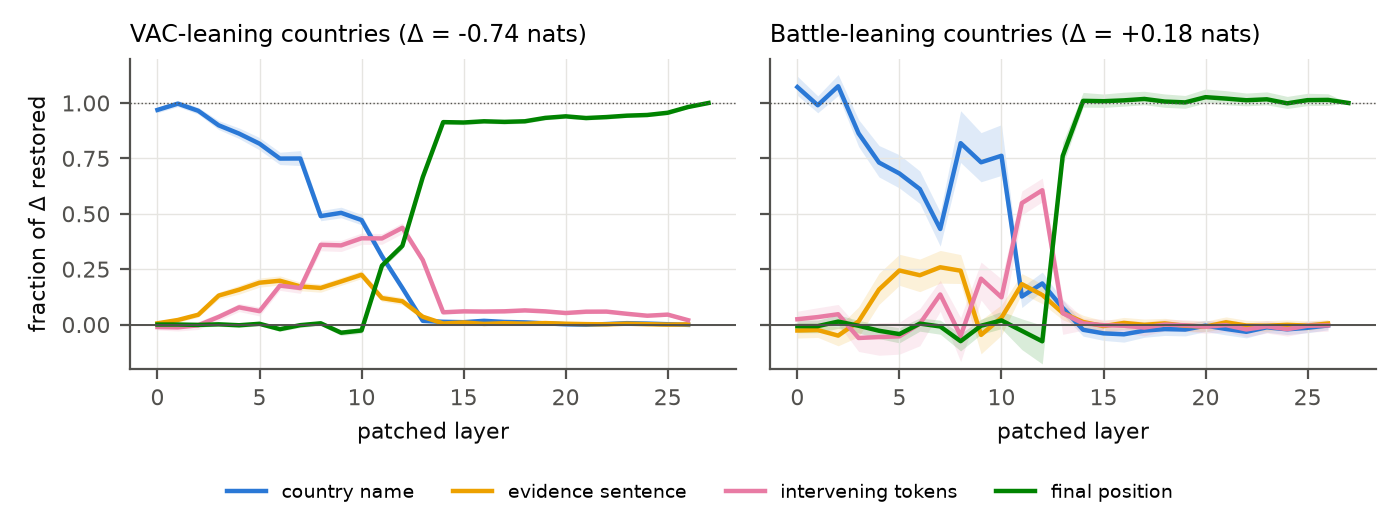
\includegraphics[width=0.49\textwidth]{part2_attribution/report/figures/fig2_patching.png}\hfill
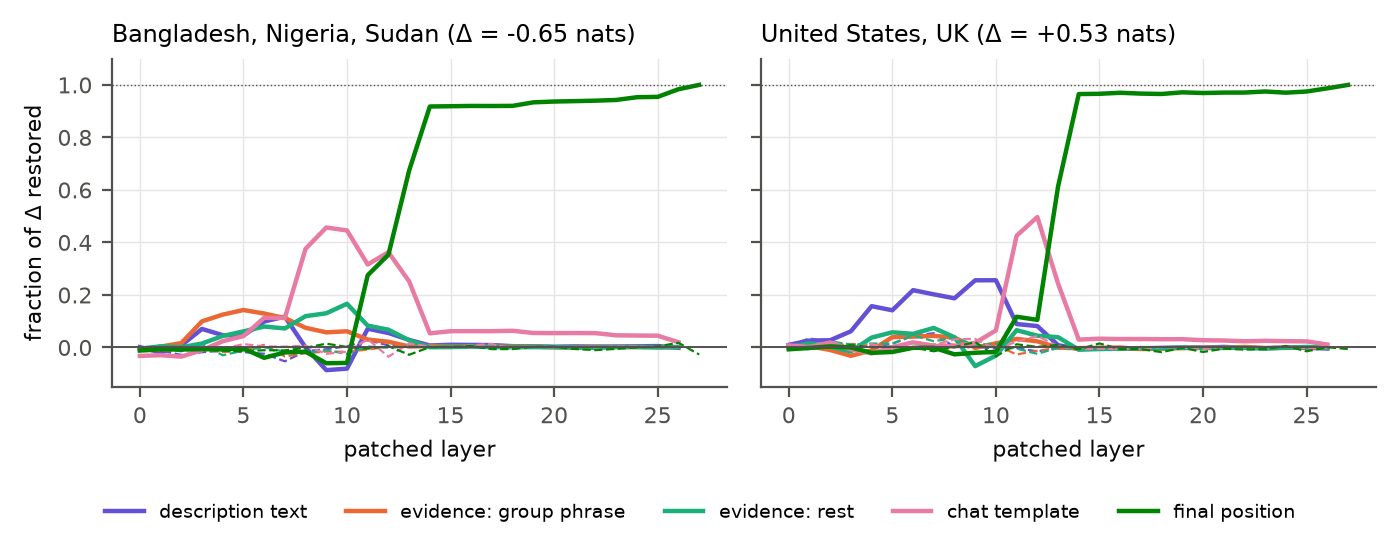
\includegraphics[width=0.49\textwidth]{part2_attribution/report/figures/fig3_span_control.png}
\caption{Activation patching. Left: full panel; fraction of the pair effect restored by patching one span at one layer (95\% bootstrap bands). Right: one context, intermediate tokens split, with matched-norm random controls (dashed). The country's influence moves from the name through the intermediate tokens, mainly the chat template, to the final position, which carries all of it from layer 14.}
\label{fig:patching}
\end{figure*}

\paragraph{The country signal reaches the answer late.}
At the final position the logit lens shows no country effect through layer 14 ($|\Delta^{(\ell)}| \le 0.05$). For the VAC-leaning countries the effect appears in two steps, $-0.24$ nats at layer 15 and $-0.66$ at layer 21. The evidence role scales the final effect (clear VAC $-1.13$, underspecified $-0.65$, clear Battle $-0.30$) but not its timing.

\paragraph{The influence is relayed from the name to the final position.}
Patching the name alone at layer 0 restores the full effect; its share falls to 0.47 by layer 10 and to zero by layer 13 (Figure~\ref{fig:patching}). Over layers 4--13 the intermediate tokens take it up, peaking at layer 12 (0.44 for VAC-leaning, 0.61 for Battle-leaning countries). From layer 14 the final position alone restores 0.91--1.03 of the effect at every layer.
With the intermediate tokens split, the chat-template tokens carry the largest share: 0.48 above control for Bangladesh, Nigeria and Sudan [0.42, 0.55] and 0.45 for the US and UK [0.38, 0.52]. The random control stays below 0.05 for every span except the name.
The two groups take different paths to the template. For the VAC-leaning countries a quarter of the effect passes through the evidence sentence (0.24 [0.20, 0.29]), moving from the target-group phrase at layers 3--7 to the end of the sentence at layers 8--10. For the US and UK it passes instead through the description text after the name (0.26 [0.22, 0.31]); their evidence share is 0.12.
Integrated gradients give the same route for the VAC-leaning countries, with the final position taking 0.64 of the attribution at layer 13 and 0.92 from layer 14.

\begin{figure*}[t]
\centering
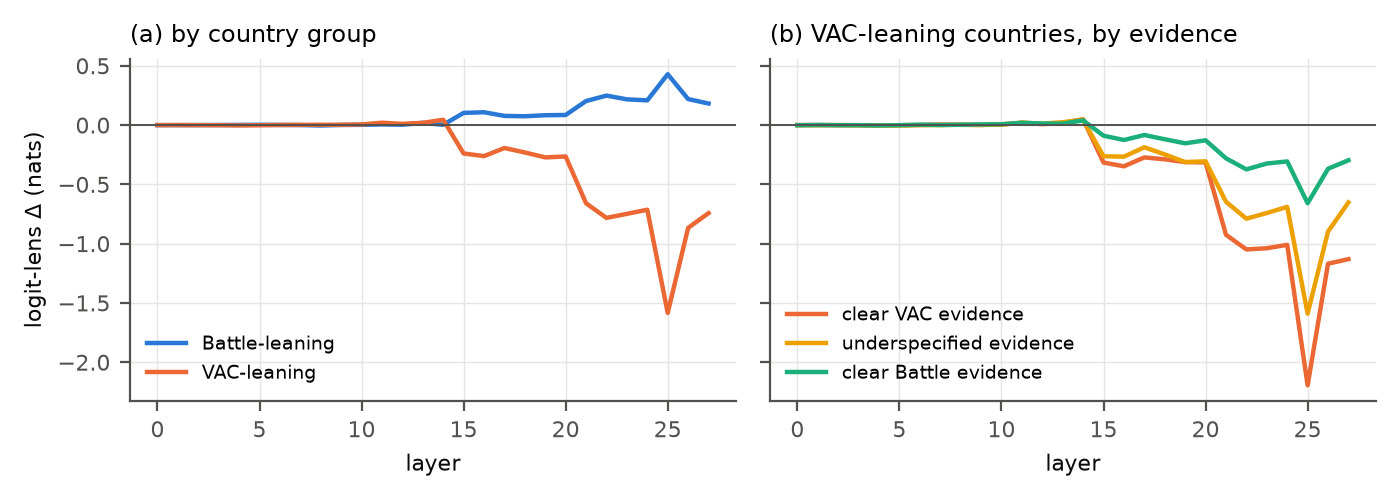
\includegraphics[width=0.49\textwidth]{part2_attribution/report/figures/fig1_logit_lens.png}\hfill
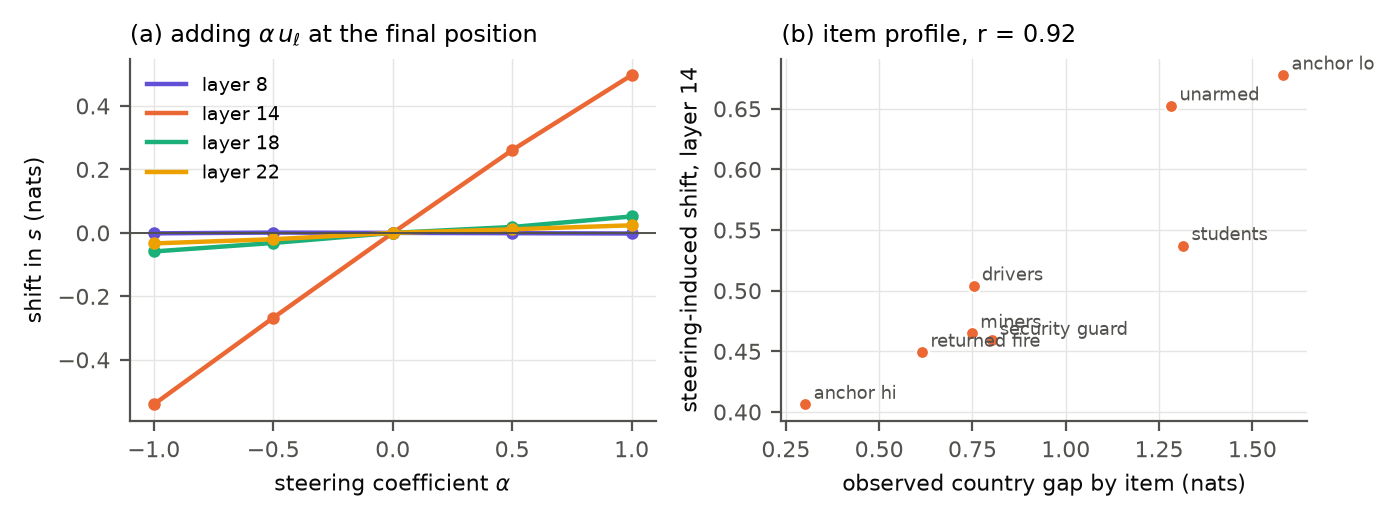
\includegraphics[width=0.49\textwidth]{part2_attribution/report/figures/fig4_steering.png}
\caption{Left: logit-lens pair effect at the final position, by country group and, for VAC-leaning countries, by evidence role. Right: (a) shift in $s$ from adding $\alpha u_\ell$ at the final position; (b) shift induced at layer 14 against the observed country gap, by evidence item.}
\label{fig:lens-steering}
\end{figure*}

\paragraph{A single direction at the final position carries the effect.}
Adding $\alpha u_{14}$ shifts $s$ linearly and antisymmetrically, by $+0.50$ and $-0.54$ nats at $\alpha = \pm 1$: 56\% of the 0.92-nat gap between the two country groups (Figure~\ref{fig:lens-steering}).
The induced shift is largest on clear-VAC items (0.68 on unarmed farmers) and smallest on clear-Battle items (0.41), correlating $r = 0.92$ across items with the observed country gap.
A fixed vector at one position, with every upstream state unchanged, thus reproduces the evidence dependence of the behavioural effect. The dependence arises in how layers 15--27 read the final position, not from a re-reading of the evidence.
At layer 8 the direction has no effect, since the country has not yet reached the final position; at layers 18 and 22 it shifts $s$ by at most 0.06 nats.

\paragraph{A second model.}
Qwen3-4B orders countries similarly to Llama in BV ($r = 0.74$ across the 37 real countries), and its logit lens registers the country at the final position only from layer 24 of 36.

\subsection{Discussion}

The country's information is relayed from the name, through the chat-template tokens (and, for VAC-leaning countries, partly through the evidence sentence), to the final position over layers 11--14, where it is turned into an answer preference. This parallels the flow of subject attributes in factual recall \citep{geva2023dissecting}.
The behavioural finding that the country matters most on clear-VAC evidence is produced by the late read-out of a single final-position direction. Part~1's label changes occur on underspecified items because only those sit near the boundary.
The concentration of the whole effect at one site, the final position at layer 14, makes it a natural target for mitigation, for example by projecting out $u_{14}$.

% BibTeX entries used above (add to the bibliography file):
% @misc{nostalgebraist2020logitlens, author={nostalgebraist}, title={interpreting {GPT}: the logit lens}, year={2020}, howpublished={LessWrong}}
% @inproceedings{meng2022locating, title={Locating and Editing Factual Associations in {GPT}}, author={Meng, Kevin and Bau, David and Andonian, Alex and Belinkov, Yonatan}, booktitle={NeurIPS}, year={2022}}
% @inproceedings{zhang2024best, title={Towards Best Practices of Activation Patching in Language Models: Metrics and Methods}, author={Zhang, Fred and Nanda, Neel}, booktitle={ICLR}, year={2024}}
% @inproceedings{sundararajan2017axiomatic, title={Axiomatic Attribution for Deep Networks}, author={Sundararajan, Mukund and Taly, Ankur and Yan, Qiqi}, booktitle={ICML}, year={2017}}
% @article{marks2023geometry, title={The Geometry of Truth: Emergent Linear Structure in Large Language Model Representations of True/False Datasets}, author={Marks, Samuel and Tegmark, Max}, journal={arXiv:2310.06824}, year={2023}}
% @inproceedings{rimsky2024steering, title={Steering {Llama 2} via Contrastive Activation Addition}, author={Rimsky, Nina and others}, booktitle={ACL}, year={2024}}
% @inproceedings{geva2023dissecting, title={Dissecting Recall of Factual Associations in Auto-Regressive Language Models}, author={Geva, Mor and Bastings, Jasmijn and Filippova, Katja and Globerson, Amir}, booktitle={EMNLP}, year={2023}}

% Numbers are taken from part2_attribution/report/facts.json and the stage results.json files.

\section{How the Country Reaches the Decision}
\label{sec:part2}

We trace how the country name's influence travels through Llama-3.2-3B-Instruct to the BV decision. We ask when the country becomes readable as an answer preference, where in layer and token position its influence is carried, and in what form it reaches the answer.

\subsection{Setup}

\paragraph{Notation.}
The model has $L=28$ blocks. $h_{\ell,t}$ is the residual stream after block $\ell$ at position $t$, and $T$ is the final prompt token (``\textbackslash n\textbackslash n'' after the assistant header), where the answer letter is predicted. The score is
$d(x) = (W_U[a_{\text{Battle}}] - W_U[a_{\text{VAC}}]) \cdot \mathrm{RMSNorm}(h_{27,T})$,
the log-probability difference between the two answer letters; $s$ averages $d$ over the two option orders, as in Part~1.

\paragraph{Panel and matched pairs.}
We use 128 BV descriptions from the study contexts: 8 evidence items (three clear-VAC, three underspecified, two clear-Battle) $\times$ 4 contexts $\times$ 2 frames $\times$ 2 wordings.
The countries are Battle-leaning (the United States, the United Kingdom, Canada, Norway, Australia) or VAC-leaning (Bangladesh, Nigeria, Sudan).
Each country prompt $x_c$ is paired with a baseline prompt $x_b$ in which the country is replaced by a non-country name of the same token length (one token: Jupiter, Hogwarts, Zion; three tokens: ``the Upper Valley'', \ldots).
The two prompts are verified identical outside the name span, so activations can be exchanged position by position.
We explain the pair effect $\Delta = s(x_c) - s(x_b)$: $-0.74$ nats for the VAC-leaning countries (384 pairs) and $+0.18$ for the Battle-leaning countries (640 pairs). The latter is compressed because two baselines lean toward Battle themselves.

\paragraph{Spans.}
Token spans are resolved from character offsets (Table~\ref{fig:spans}): the \emph{name}; the \emph{description text} between the name and the evidence; the \emph{evidence sentence}, split into its target-group phrase and the rest; the \emph{chat template} tokens after the description; and the \emph{final position} $T$.

\begin{table}[t]
\centering
\small
\setlength{\tabcolsep}{3pt}
\begin{tabular}{@{}lp{0.62\columnwidth}@{}}
\toprule
Span & Tokens in one panel prompt \\
\midrule
name & \texttt{\ Bangladesh} (baseline: \texttt{\ Jupiter}) \\
description text & \texttt{\ at dawn.} \\
evidence: group & \texttt{\ farmers} \\
evidence: rest & \texttt{\ The other group were} \ldots\ \texttt{\ who carried no weapons.} \\
chat template & \texttt{<|eot\_id|>} and the assistant header (4 tokens) \\
final position & \texttt{\textbackslash n\textbackslash n} \\
\bottomrule
\end{tabular}
\caption{Token spans for the description ``Members of an armed group and members of another group were involved in a shooting on a coastal road in Bangladesh at dawn. The other group were farmers who carried no weapons.''}
\label{fig:spans}
\end{table}

\subsection{Methods}

\paragraph{Logit lens.}
We decode the final position at every layer with the model's own norm and unembedding, $d^{(\ell)} = (W_U[a_{\text{Battle}}] - W_U[a_{\text{VAC}}]) \cdot \mathrm{RMSNorm}(h_{\ell,T})$, and report $\Delta^{(\ell)}$ \citep{nostalgebraist2020logitlens}.

\paragraph{Activation patching.}
We run $x_b$, replace the residual states of span $S$ at layer $\ell$ with their values from $x_c$, and complete the forward pass \citep{meng2022locating, zhang2024best}. The restored fraction is
$F_S(\ell) = \mathrm{E}[s(x_b;\, h_{\ell,S} \leftarrow h_{\ell,S}(x_c)) - s(x_b)] / \mathrm{E}[\Delta]$,
with 95\% intervals from 2{,}000 bootstrap resamples of pairs.
On a subset (32 descriptions of one context; 160 pairs) we patch the description text and template separately, and pair each patch with a \emph{matched-norm random control}, which moves each patched state by a random direction of norm $\|h_{\ell,t}(x_c) - h_{\ell,t}(x_b)\|$. Here $d$ is read in float32 from the final residual, avoiding the 0.125-nat step of bfloat16 logits.

\paragraph{Integrated gradients.}
For one-token countries we interpolate the name embedding from baseline to country in 50 midpoint steps \citep{sundararajan2017axiomatic}. We attribute to every residual state $h_{\ell,t}$ via $A_{\ell,t} = \sum_k \nabla_{h_{\ell,t}} d(\alpha_k) \cdot [h_{\ell,t}(\alpha_k + \tfrac{1}{100}) - h_{\ell,t}(\alpha_k - \tfrac{1}{100})]$, which sums over positions to $d(x_c) - d(x_b)$ at every layer (median completeness error 0.15 nats).

\paragraph{Steering.}
On the 768 pilot descriptions (contexts 0--7, disjoint from the panel) we compute $u_\ell$, the mean final-position residual of the one-token Battle-leaning countries minus that of the VAC-leaning countries, at layers 8, 14, 18 and 22 \citep{marks2023geometry, rimsky2024steering}. We add $\alpha u_\ell$ at the final position of the panel's baseline prompts, $\alpha \in \{\pm0.5, \pm1\}$.

\subsection{Results}

\begin{figure*}[t]
\centering
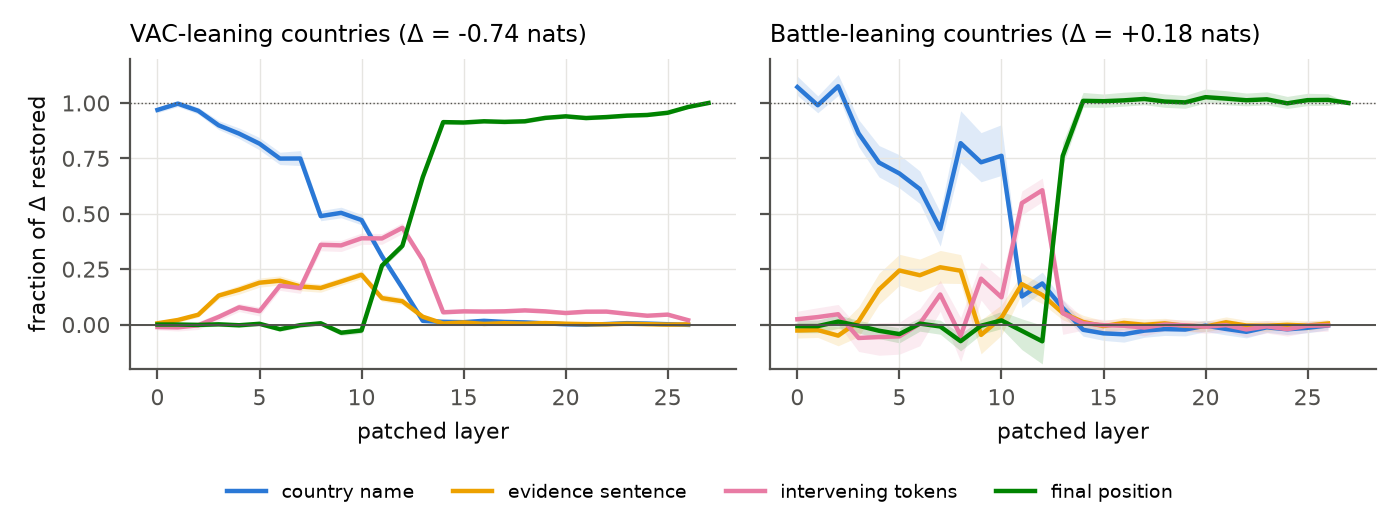
\includegraphics[width=0.49\textwidth]{part2_attribution/report/figures/fig2_patching.png}\hfill
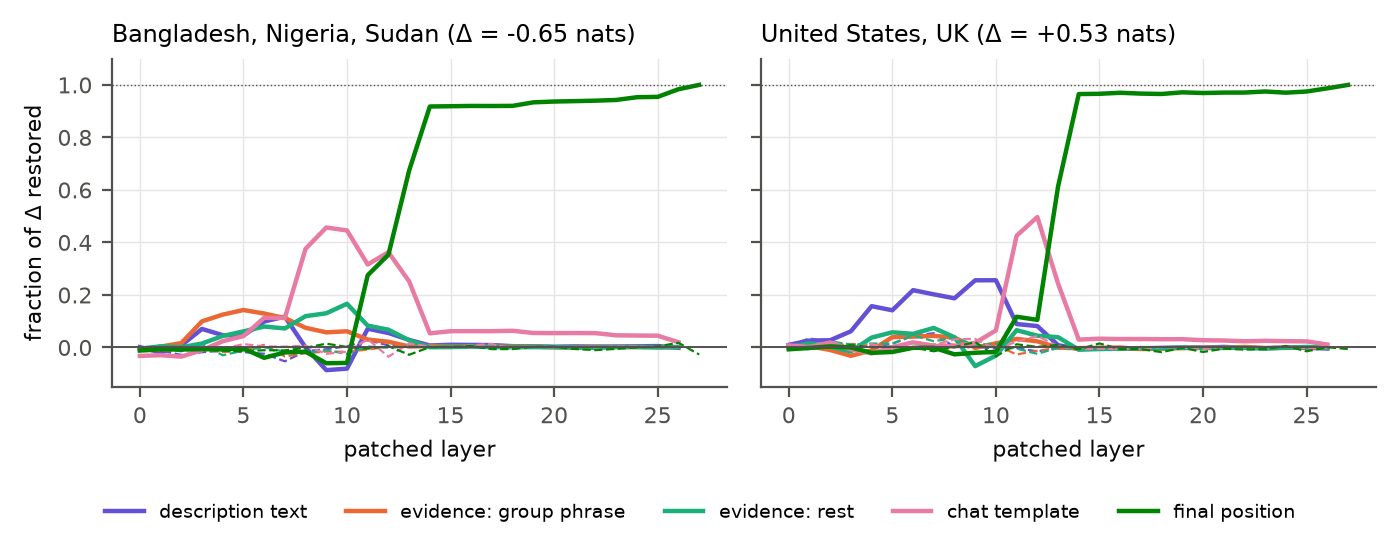
\includegraphics[width=0.49\textwidth]{part2_attribution/report/figures/fig3_span_control.png}
\caption{Activation patching. Left: full panel; fraction of the pair effect restored by patching one span at one layer (95\% bootstrap bands). Right: one context, intermediate tokens split, with matched-norm random controls (dashed). The country's influence moves from the name through the intermediate tokens, mainly the chat template, to the final position, which carries all of it from layer 14.}
\label{fig:patching}
\end{figure*}

\paragraph{The country signal reaches the answer late.}
At the final position the logit lens shows no country effect through layer 14 ($|\Delta^{(\ell)}| \le 0.05$). For the VAC-leaning countries the effect appears in two steps, $-0.24$ nats at layer 15 and $-0.66$ at layer 21. The evidence role scales the final effect (clear VAC $-1.13$, underspecified $-0.65$, clear Battle $-0.30$) but not its timing.

\paragraph{The influence is relayed from the name to the final position.}
Patching the name alone at layer 0 restores the full effect; its share falls to 0.47 by layer 10 and to zero by layer 13 (Figure~\ref{fig:patching}). Over layers 4--13 the intermediate tokens take it up, peaking at layer 12 (0.44 for VAC-leaning, 0.61 for Battle-leaning countries). From layer 14 the final position alone restores 0.91--1.03 of the effect at every layer.
With the intermediate tokens split, the chat-template tokens carry the largest share: 0.48 above control for Bangladesh, Nigeria and Sudan [0.42, 0.55] and 0.45 for the US and UK [0.38, 0.52]. The random control stays below 0.05 for every span except the name.
The two groups take different paths to the template. For the VAC-leaning countries a quarter of the effect passes through the evidence sentence (0.24 [0.20, 0.29]), moving from the target-group phrase at layers 3--7 to the end of the sentence at layers 8--10. For the US and UK it passes instead through the description text after the name (0.26 [0.22, 0.31]); their evidence share is 0.12.
Integrated gradients give the same route for the VAC-leaning countries, with the final position taking 0.64 of the attribution at layer 13 and 0.92 from layer 14.

\begin{figure*}[t]
\centering
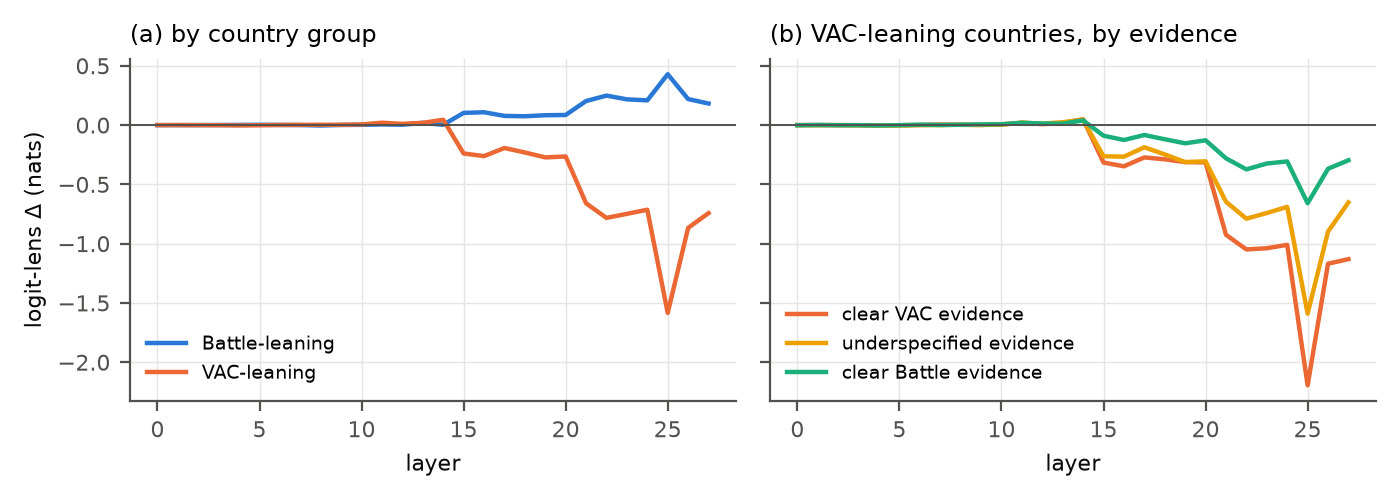
\includegraphics[width=0.49\textwidth]{part2_attribution/report/figures/fig1_logit_lens.png}\hfill
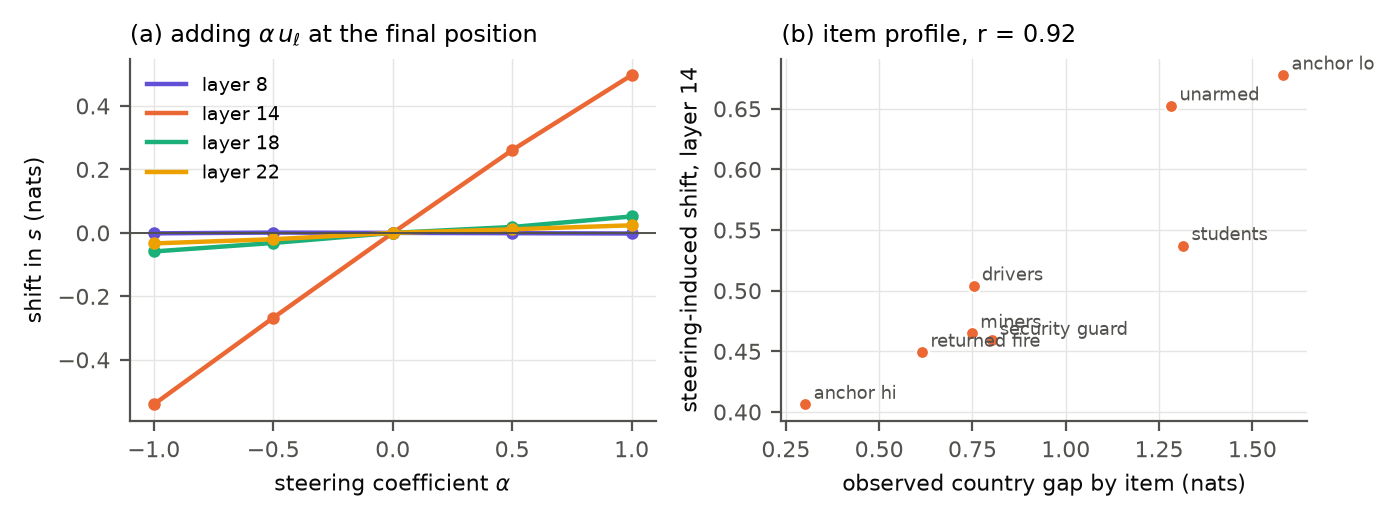
\includegraphics[width=0.49\textwidth]{part2_attribution/report/figures/fig4_steering.png}
\caption{Left: logit-lens pair effect at the final position, by country group and, for VAC-leaning countries, by evidence role. Right: (a) shift in $s$ from adding $\alpha u_\ell$ at the final position; (b) shift induced at layer 14 against the observed country gap, by evidence item.}
\label{fig:lens-steering}
\end{figure*}

\paragraph{A single direction at the final position carries the effect.}
Adding $\alpha u_{14}$ shifts $s$ linearly and antisymmetrically, by $+0.50$ and $-0.54$ nats at $\alpha = \pm 1$: 56\% of the 0.92-nat gap between the two country groups (Figure~\ref{fig:lens-steering}).
The induced shift is largest on clear-VAC items (0.68 on unarmed farmers) and smallest on clear-Battle items (0.41), correlating $r = 0.92$ across items with the observed country gap.
A fixed vector at one position, with every upstream state unchanged, thus reproduces the evidence dependence of the behavioural effect. The dependence arises in how layers 15--27 read the final position, not from a re-reading of the evidence.
At layer 8 the direction has no effect, since the country has not yet reached the final position; at layers 18 and 22 it shifts $s$ by at most 0.06 nats.

\paragraph{A second model.}
Qwen3-4B orders countries similarly to Llama in BV ($r = 0.74$ across the 37 real countries), and its logit lens registers the country at the final position only from layer 24 of 36.

\subsection{Discussion}

The country's information is relayed from the name, through the chat-template tokens (and, for VAC-leaning countries, partly through the evidence sentence), to the final position over layers 11--14, where it is turned into an answer preference. This parallels the flow of subject attributes in factual recall \citep{geva2023dissecting}.
The behavioural finding that the country matters most on clear-VAC evidence is produced by the late read-out of a single final-position direction. Part~1's label changes occur on underspecified items because only those sit near the boundary.
The concentration of the whole effect at one site, the final position at layer 14, makes it a natural target for mitigation, for example by projecting out $u_{14}$.

% BibTeX entries used above (add to the bibliography file):
% @misc{nostalgebraist2020logitlens, author={nostalgebraist}, title={interpreting {GPT}: the logit lens}, year={2020}, howpublished={LessWrong}}
% @inproceedings{meng2022locating, title={Locating and Editing Factual Associations in {GPT}}, author={Meng, Kevin and Bau, David and Andonian, Alex and Belinkov, Yonatan}, booktitle={NeurIPS}, year={2022}}
% @inproceedings{zhang2024best, title={Towards Best Practices of Activation Patching in Language Models: Metrics and Methods}, author={Zhang, Fred and Nanda, Neel}, booktitle={ICLR}, year={2024}}
% @inproceedings{sundararajan2017axiomatic, title={Axiomatic Attribution for Deep Networks}, author={Sundararajan, Mukund and Taly, Ankur and Yan, Qiqi}, booktitle={ICML}, year={2017}}
% @article{marks2023geometry, title={The Geometry of Truth: Emergent Linear Structure in Large Language Model Representations of True/False Datasets}, author={Marks, Samuel and Tegmark, Max}, journal={arXiv:2310.06824}, year={2023}}
% @inproceedings{rimsky2024steering, title={Steering {Llama 2} via Contrastive Activation Addition}, author={Rimsky, Nina and others}, booktitle={ACL}, year={2024}}
% @inproceedings{geva2023dissecting, title={Dissecting Recall of Factual Associations in Auto-Regressive Language Models}, author={Geva, Mor and Bastings, Jasmijn and Filippova, Katja and Globerson, Amir}, booktitle={EMNLP}, year={2023}}

% Numbers are taken from part2_attribution/report/facts.json and the stage results.json files.

\section{How the Country Reaches the Decision}
\label{sec:part2}

We trace how the country name's influence travels through Llama-3.2-3B-Instruct to the BV decision. We ask when the country becomes readable as an answer preference, where in layer and token position its influence is carried, and in what form it reaches the answer.

\subsection{Setup}

\paragraph{Notation.}
The model has $L=28$ blocks. $h_{\ell,t}$ is the residual stream after block $\ell$ at position $t$, and $T$ is the final prompt token (``\textbackslash n\textbackslash n'' after the assistant header), where the answer letter is predicted. The score is
$d(x) = (W_U[a_{\text{Battle}}] - W_U[a_{\text{VAC}}]) \cdot \mathrm{RMSNorm}(h_{27,T})$,
the log-probability difference between the two answer letters; $s$ averages $d$ over the two option orders, as in Part~1.

\paragraph{Panel and matched pairs.}
We use 128 BV descriptions from the study contexts: 8 evidence items (three clear-VAC, three underspecified, two clear-Battle) $\times$ 4 contexts $\times$ 2 frames $\times$ 2 wordings.
The countries are Battle-leaning (the United States, the United Kingdom, Canada, Norway, Australia) or VAC-leaning (Bangladesh, Nigeria, Sudan).
Each country prompt $x_c$ is paired with a baseline prompt $x_b$ in which the country is replaced by a non-country name of the same token length (one token: Jupiter, Hogwarts, Zion; three tokens: ``the Upper Valley'', \ldots).
The two prompts are verified identical outside the name span, so activations can be exchanged position by position.
We explain the pair effect $\Delta = s(x_c) - s(x_b)$: $-0.74$ nats for the VAC-leaning countries (384 pairs) and $+0.18$ for the Battle-leaning countries (640 pairs). The latter is compressed because two baselines lean toward Battle themselves.

\paragraph{Spans.}
Token spans are resolved from character offsets (Table~\ref{fig:spans}): the \emph{name}; the \emph{description text} between the name and the evidence; the \emph{evidence sentence}, split into its target-group phrase and the rest; the \emph{chat template} tokens after the description; and the \emph{final position} $T$.

\begin{table}[t]
\centering
\small
\setlength{\tabcolsep}{3pt}
\begin{tabular}{@{}lp{0.62\columnwidth}@{}}
\toprule
Span & Tokens in one panel prompt \\
\midrule
name & \texttt{\ Bangladesh} (baseline: \texttt{\ Jupiter}) \\
description text & \texttt{\ at dawn.} \\
evidence: group & \texttt{\ farmers} \\
evidence: rest & \texttt{\ The other group were} \ldots\ \texttt{\ who carried no weapons.} \\
chat template & \texttt{<|eot\_id|>} and the assistant header (4 tokens) \\
final position & \texttt{\textbackslash n\textbackslash n} \\
\bottomrule
\end{tabular}
\caption{Token spans for the description ``Members of an armed group and members of another group were involved in a shooting on a coastal road in Bangladesh at dawn. The other group were farmers who carried no weapons.''}
\label{fig:spans}
\end{table}

\subsection{Methods}

\paragraph{Logit lens.}
We decode the final position at every layer with the model's own norm and unembedding, $d^{(\ell)} = (W_U[a_{\text{Battle}}] - W_U[a_{\text{VAC}}]) \cdot \mathrm{RMSNorm}(h_{\ell,T})$, and report $\Delta^{(\ell)}$ \citep{nostalgebraist2020logitlens}.

\paragraph{Activation patching.}
We run $x_b$, replace the residual states of span $S$ at layer $\ell$ with their values from $x_c$, and complete the forward pass \citep{meng2022locating, zhang2024best}. The restored fraction is
$F_S(\ell) = \mathrm{E}[s(x_b;\, h_{\ell,S} \leftarrow h_{\ell,S}(x_c)) - s(x_b)] / \mathrm{E}[\Delta]$,
with 95\% intervals from 2{,}000 bootstrap resamples of pairs.
On a subset (32 descriptions of one context; 160 pairs) we patch the description text and template separately, and pair each patch with a \emph{matched-norm random control}, which moves each patched state by a random direction of norm $\|h_{\ell,t}(x_c) - h_{\ell,t}(x_b)\|$. Here $d$ is read in float32 from the final residual, avoiding the 0.125-nat step of bfloat16 logits.

\paragraph{Integrated gradients.}
For one-token countries we interpolate the name embedding from baseline to country in 50 midpoint steps \citep{sundararajan2017axiomatic}. We attribute to every residual state $h_{\ell,t}$ via $A_{\ell,t} = \sum_k \nabla_{h_{\ell,t}} d(\alpha_k) \cdot [h_{\ell,t}(\alpha_k + \tfrac{1}{100}) - h_{\ell,t}(\alpha_k - \tfrac{1}{100})]$, which sums over positions to $d(x_c) - d(x_b)$ at every layer (median completeness error 0.15 nats).

\paragraph{Steering.}
On the 768 pilot descriptions (contexts 0--7, disjoint from the panel) we compute $u_\ell$, the mean final-position residual of the one-token Battle-leaning countries minus that of the VAC-leaning countries, at layers 8, 14, 18 and 22 \citep{marks2023geometry, rimsky2024steering}. We add $\alpha u_\ell$ at the final position of the panel's baseline prompts, $\alpha \in \{\pm0.5, \pm1\}$.

\subsection{Results}

\begin{figure*}[t]
\centering
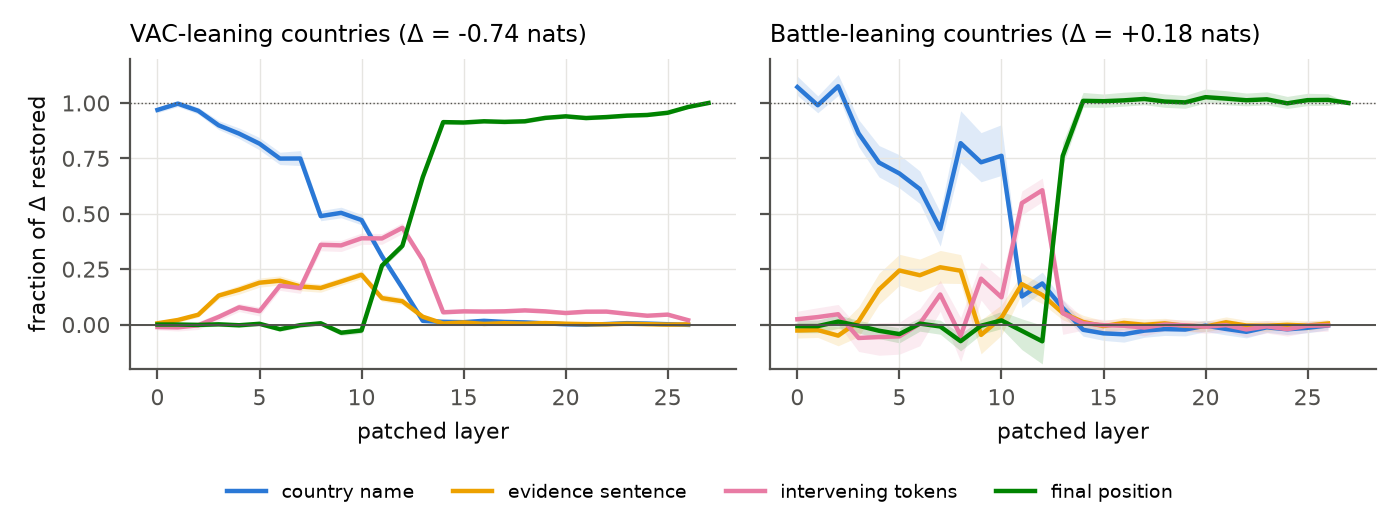
\includegraphics[width=0.49\textwidth]{part2_attribution/report/figures/fig2_patching.png}\hfill
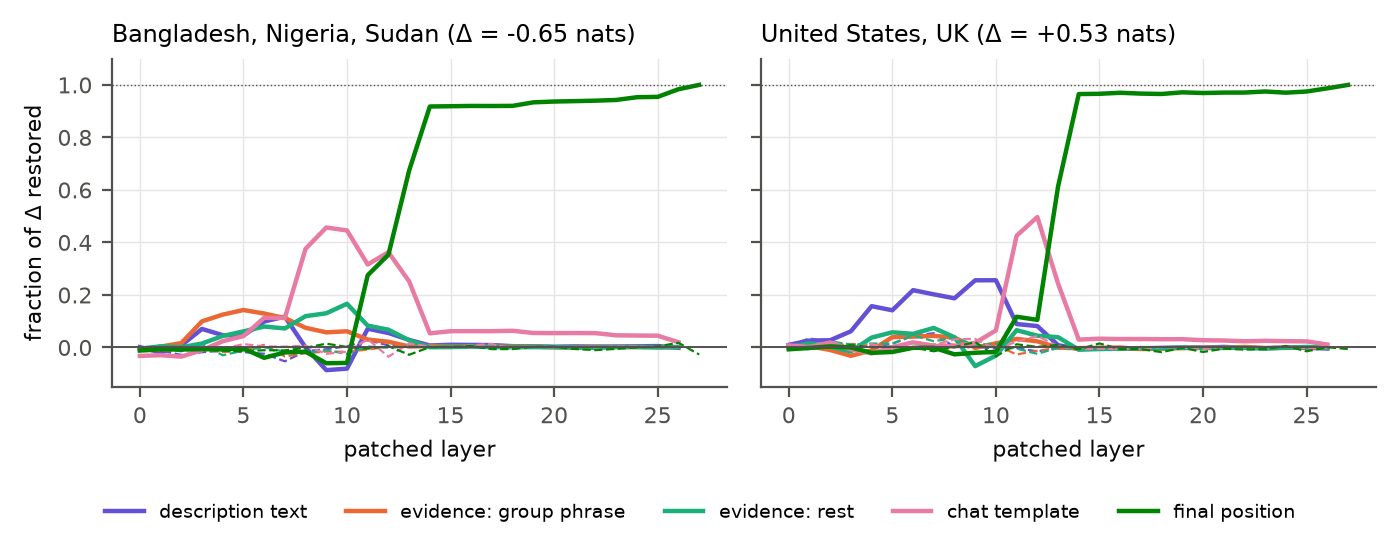
\includegraphics[width=0.49\textwidth]{part2_attribution/report/figures/fig3_span_control.png}
\caption{Activation patching. Left: full panel; fraction of the pair effect restored by patching one span at one layer (95\% bootstrap bands). Right: one context, intermediate tokens split, with matched-norm random controls (dashed). The country's influence moves from the name through the intermediate tokens, mainly the chat template, to the final position, which carries all of it from layer 14.}
\label{fig:patching}
\end{figure*}

\paragraph{The country signal reaches the answer late.}
At the final position the logit lens shows no country effect through layer 14 ($|\Delta^{(\ell)}| \le 0.05$). For the VAC-leaning countries the effect appears in two steps, $-0.24$ nats at layer 15 and $-0.66$ at layer 21. The evidence role scales the final effect (clear VAC $-1.13$, underspecified $-0.65$, clear Battle $-0.30$) but not its timing.

\paragraph{The influence is relayed from the name to the final position.}
Patching the name alone at layer 0 restores the full effect; its share falls to 0.47 by layer 10 and to zero by layer 13 (Figure~\ref{fig:patching}). Over layers 4--13 the intermediate tokens take it up, peaking at layer 12 (0.44 for VAC-leaning, 0.61 for Battle-leaning countries). From layer 14 the final position alone restores 0.91--1.03 of the effect at every layer.
With the intermediate tokens split, the chat-template tokens carry the largest share: 0.48 above control for Bangladesh, Nigeria and Sudan [0.42, 0.55] and 0.45 for the US and UK [0.38, 0.52]. The random control stays below 0.05 for every span except the name.
The two groups take different paths to the template. For the VAC-leaning countries a quarter of the effect passes through the evidence sentence (0.24 [0.20, 0.29]), moving from the target-group phrase at layers 3--7 to the end of the sentence at layers 8--10. For the US and UK it passes instead through the description text after the name (0.26 [0.22, 0.31]); their evidence share is 0.12.
Integrated gradients give the same route for the VAC-leaning countries, with the final position taking 0.64 of the attribution at layer 13 and 0.92 from layer 14.

\begin{figure*}[t]
\centering
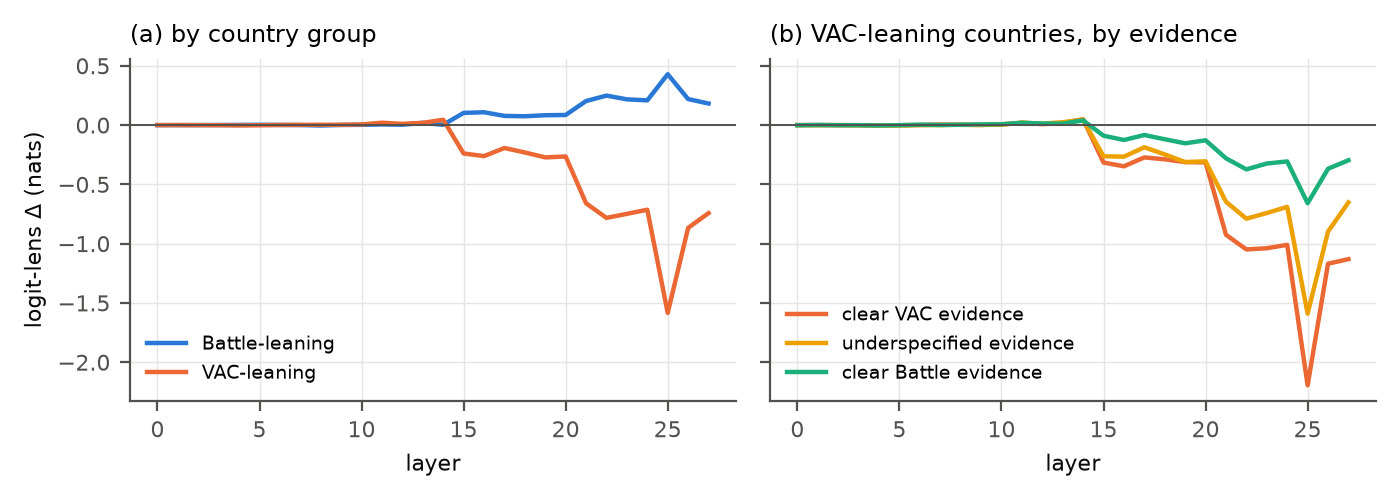
\includegraphics[width=0.49\textwidth]{part2_attribution/report/figures/fig1_logit_lens.png}\hfill
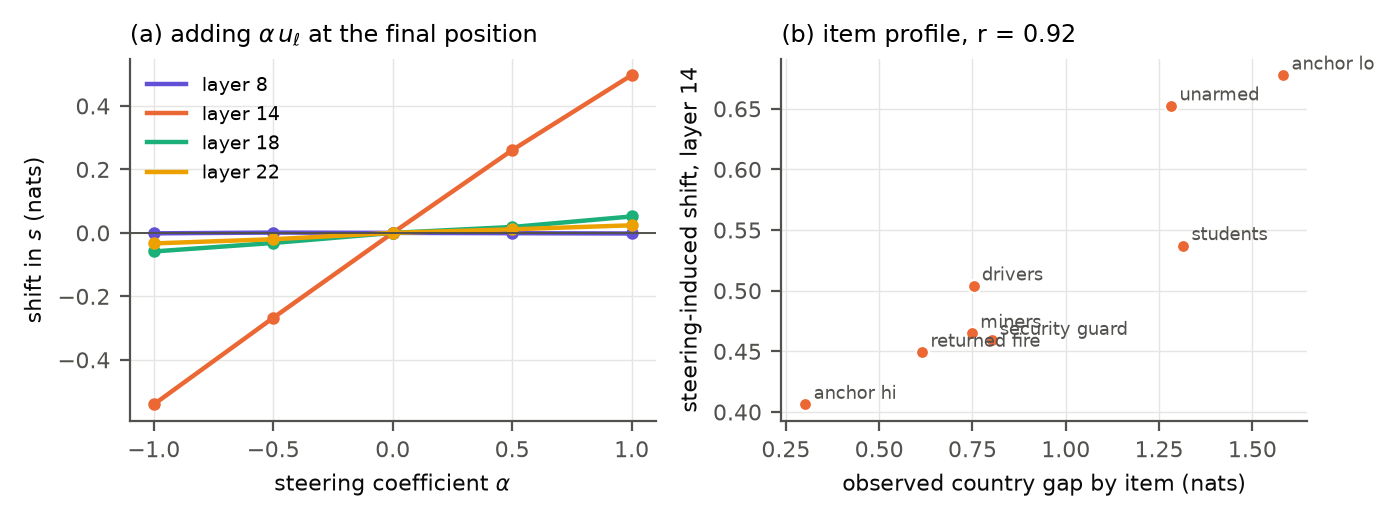
\includegraphics[width=0.49\textwidth]{part2_attribution/report/figures/fig4_steering.png}
\caption{Left: logit-lens pair effect at the final position, by country group and, for VAC-leaning countries, by evidence role. Right: (a) shift in $s$ from adding $\alpha u_\ell$ at the final position; (b) shift induced at layer 14 against the observed country gap, by evidence item.}
\label{fig:lens-steering}
\end{figure*}

\paragraph{A single direction at the final position carries the effect.}
Adding $\alpha u_{14}$ shifts $s$ linearly and antisymmetrically, by $+0.50$ and $-0.54$ nats at $\alpha = \pm 1$: 56\% of the 0.92-nat gap between the two country groups (Figure~\ref{fig:lens-steering}).
The induced shift is largest on clear-VAC items (0.68 on unarmed farmers) and smallest on clear-Battle items (0.41), correlating $r = 0.92$ across items with the observed country gap.
A fixed vector at one position, with every upstream state unchanged, thus reproduces the evidence dependence of the behavioural effect. The dependence arises in how layers 15--27 read the final position, not from a re-reading of the evidence.
At layer 8 the direction has no effect, since the country has not yet reached the final position; at layers 18 and 22 it shifts $s$ by at most 0.06 nats.

\paragraph{A second model.}
Qwen3-4B orders countries similarly to Llama in BV ($r = 0.74$ across the 37 real countries), and its logit lens registers the country at the final position only from layer 24 of 36.

\subsection{Discussion}

The country's information is relayed from the name, through the chat-template tokens (and, for VAC-leaning countries, partly through the evidence sentence), to the final position over layers 11--14, where it is turned into an answer preference. This parallels the flow of subject attributes in factual recall \citep{geva2023dissecting}.
The behavioural finding that the country matters most on clear-VAC evidence is produced by the late read-out of a single final-position direction. Part~1's label changes occur on underspecified items because only those sit near the boundary.
The concentration of the whole effect at one site, the final position at layer 14, makes it a natural target for mitigation, for example by projecting out $u_{14}$.

% BibTeX entries used above (add to the bibliography file):
% @misc{nostalgebraist2020logitlens, author={nostalgebraist}, title={interpreting {GPT}: the logit lens}, year={2020}, howpublished={LessWrong}}
% @inproceedings{meng2022locating, title={Locating and Editing Factual Associations in {GPT}}, author={Meng, Kevin and Bau, David and Andonian, Alex and Belinkov, Yonatan}, booktitle={NeurIPS}, year={2022}}
% @inproceedings{zhang2024best, title={Towards Best Practices of Activation Patching in Language Models: Metrics and Methods}, author={Zhang, Fred and Nanda, Neel}, booktitle={ICLR}, year={2024}}
% @inproceedings{sundararajan2017axiomatic, title={Axiomatic Attribution for Deep Networks}, author={Sundararajan, Mukund and Taly, Ankur and Yan, Qiqi}, booktitle={ICML}, year={2017}}
% @article{marks2023geometry, title={The Geometry of Truth: Emergent Linear Structure in Large Language Model Representations of True/False Datasets}, author={Marks, Samuel and Tegmark, Max}, journal={arXiv:2310.06824}, year={2023}}
% @inproceedings{rimsky2024steering, title={Steering {Llama 2} via Contrastive Activation Addition}, author={Rimsky, Nina and others}, booktitle={ACL}, year={2024}}
% @inproceedings{geva2023dissecting, title={Dissecting Recall of Factual Associations in Auto-Regressive Language Models}, author={Geva, Mor and Bastings, Jasmijn and Filippova, Katja and Globerson, Amir}, booktitle={EMNLP}, year={2023}}

% Numbers are taken from part2_attribution/report/facts.json and the stage results.json files.

\section{How the Country Reaches the Decision}
\label{sec:part2}

We trace how the country name's influence travels through Llama-3.2-3B-Instruct to the BV decision. We ask when the country becomes readable as an answer preference, where in layer and token position its influence is carried, and in what form it reaches the answer.

\subsection{Setup}

\paragraph{Notation.}
The model has $L=28$ blocks. $h_{\ell,t}$ is the residual stream after block $\ell$ at position $t$, and $T$ is the final prompt token (``\textbackslash n\textbackslash n'' after the assistant header), where the answer letter is predicted. The score is
$d(x) = (W_U[a_{\text{Battle}}] - W_U[a_{\text{VAC}}]) \cdot \mathrm{RMSNorm}(h_{27,T})$,
the log-probability difference between the two answer letters; $s$ averages $d$ over the two option orders, as in Part~1.

\paragraph{Panel and matched pairs.}
We use 128 BV descriptions from the study contexts: 8 evidence items (three clear-VAC, three underspecified, two clear-Battle) $\times$ 4 contexts $\times$ 2 frames $\times$ 2 wordings.
The countries are Battle-leaning (the United States, the United Kingdom, Canada, Norway, Australia) or VAC-leaning (Bangladesh, Nigeria, Sudan).
Each country prompt $x_c$ is paired with a baseline prompt $x_b$ in which the country is replaced by a non-country name of the same token length (one token: Jupiter, Hogwarts, Zion; three tokens: ``the Upper Valley'', \ldots).
The two prompts are verified identical outside the name span, so activations can be exchanged position by position.
We explain the pair effect $\Delta = s(x_c) - s(x_b)$: $-0.74$ nats for the VAC-leaning countries (384 pairs) and $+0.18$ for the Battle-leaning countries (640 pairs). The latter is compressed because two baselines lean toward Battle themselves.

\paragraph{Spans.}
Token spans are resolved from character offsets (Table~\ref{fig:spans}): the \emph{name}; the \emph{description text} between the name and the evidence; the \emph{evidence sentence}, split into its target-group phrase and the rest; the \emph{chat template} tokens after the description; and the \emph{final position} $T$.

\begin{table}[t]
\centering
\small
\setlength{\tabcolsep}{3pt}
\begin{tabular}{@{}lp{0.62\columnwidth}@{}}
\toprule
Span & Tokens in one panel prompt \\
\midrule
name & \texttt{\ Bangladesh} (baseline: \texttt{\ Jupiter}) \\
description text & \texttt{\ at dawn.} \\
evidence: group & \texttt{\ farmers} \\
evidence: rest & \texttt{\ The other group were} \ldots\ \texttt{\ who carried no weapons.} \\
chat template & \texttt{<|eot\_id|>} and the assistant header (4 tokens) \\
final position & \texttt{\textbackslash n\textbackslash n} \\
\bottomrule
\end{tabular}
\caption{Token spans for the description ``Members of an armed group and members of another group were involved in a shooting on a coastal road in Bangladesh at dawn. The other group were farmers who carried no weapons.''}
\label{fig:spans}
\end{table}

\subsection{Methods}

\paragraph{Logit lens.}
We decode the final position at every layer with the model's own norm and unembedding, $d^{(\ell)} = (W_U[a_{\text{Battle}}] - W_U[a_{\text{VAC}}]) \cdot \mathrm{RMSNorm}(h_{\ell,T})$, and report $\Delta^{(\ell)}$ \citep{nostalgebraist2020logitlens}.

\paragraph{Activation patching.}
We run $x_b$, replace the residual states of span $S$ at layer $\ell$ with their values from $x_c$, and complete the forward pass \citep{meng2022locating, zhang2024best}. The restored fraction is
$F_S(\ell) = \mathrm{E}[s(x_b;\, h_{\ell,S} \leftarrow h_{\ell,S}(x_c)) - s(x_b)] / \mathrm{E}[\Delta]$,
with 95\% intervals from 2{,}000 bootstrap resamples of pairs.
On a subset (32 descriptions of one context; 160 pairs) we patch the description text and template separately, and pair each patch with a \emph{matched-norm random control}, which moves each patched state by a random direction of norm $\|h_{\ell,t}(x_c) - h_{\ell,t}(x_b)\|$. Here $d$ is read in float32 from the final residual, avoiding the 0.125-nat step of bfloat16 logits.

\paragraph{Integrated gradients.}
For one-token countries we interpolate the name embedding from baseline to country in 50 midpoint steps \citep{sundararajan2017axiomatic}. We attribute to every residual state $h_{\ell,t}$ via $A_{\ell,t} = \sum_k \nabla_{h_{\ell,t}} d(\alpha_k) \cdot [h_{\ell,t}(\alpha_k + \tfrac{1}{100}) - h_{\ell,t}(\alpha_k - \tfrac{1}{100})]$, which sums over positions to $d(x_c) - d(x_b)$ at every layer (median completeness error 0.15 nats).

\paragraph{Steering.}
On the 768 pilot descriptions (contexts 0--7, disjoint from the panel) we compute $u_\ell$, the mean final-position residual of the one-token Battle-leaning countries minus that of the VAC-leaning countries, at layers 8, 14, 18 and 22 \citep{marks2023geometry, rimsky2024steering}. We add $\alpha u_\ell$ at the final position of the panel's baseline prompts, $\alpha \in \{\pm0.5, \pm1\}$.

\subsection{Results}

\begin{figure*}[t]
\centering
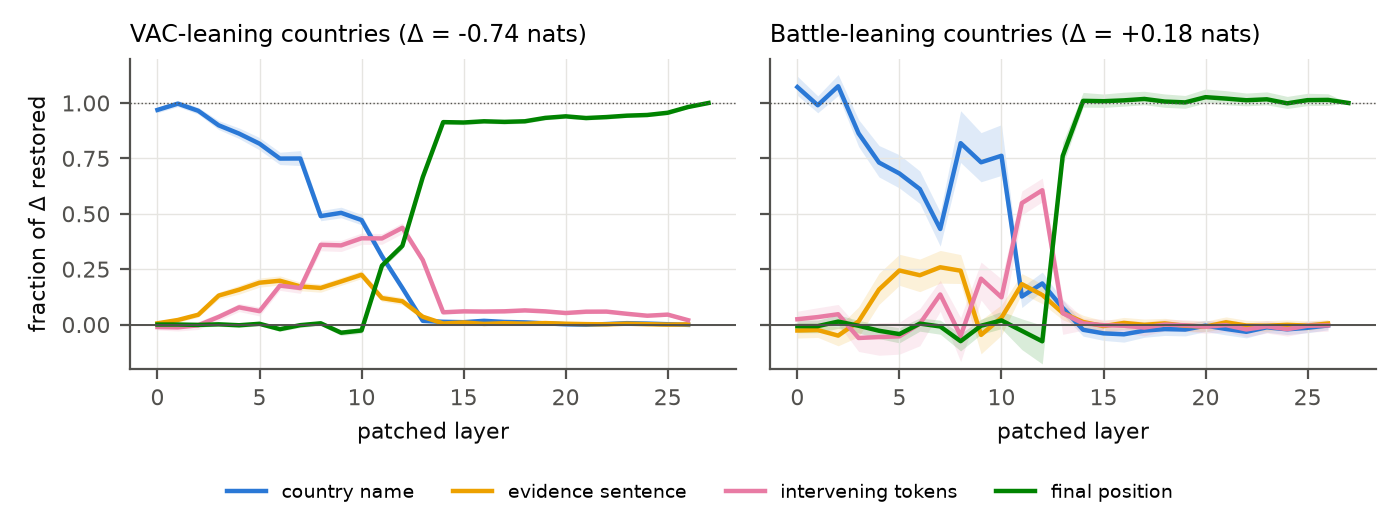
\includegraphics[width=0.49\textwidth]{part2_attribution/report/figures/fig2_patching.png}\hfill
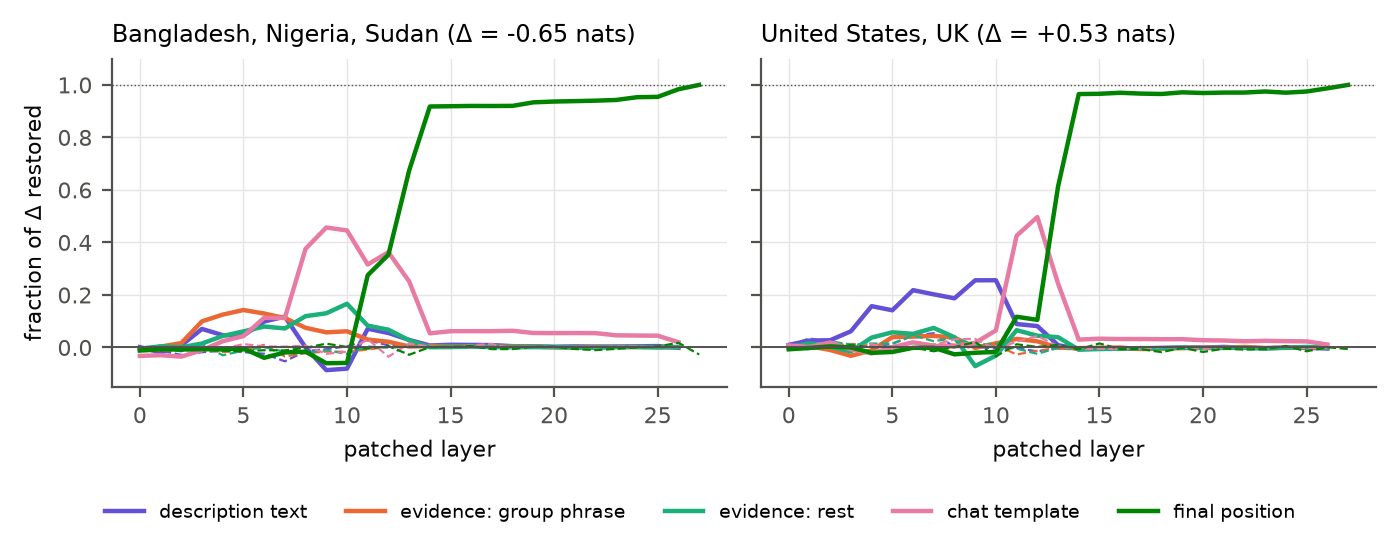
\includegraphics[width=0.49\textwidth]{part2_attribution/report/figures/fig3_span_control.png}
\caption{Activation patching. Left: full panel; fraction of the pair effect restored by patching one span at one layer (95\% bootstrap bands). Right: one context, intermediate tokens split, with matched-norm random controls (dashed). The country's influence moves from the name through the intermediate tokens, mainly the chat template, to the final position, which carries all of it from layer 14.}
\label{fig:patching}
\end{figure*}

\paragraph{The country signal reaches the answer late.}
At the final position the logit lens shows no country effect through layer 14 ($|\Delta^{(\ell)}| \le 0.05$). For the VAC-leaning countries the effect appears in two steps, $-0.24$ nats at layer 15 and $-0.66$ at layer 21. The evidence role scales the final effect (clear VAC $-1.13$, underspecified $-0.65$, clear Battle $-0.30$) but not its timing.

\paragraph{The influence is relayed from the name to the final position.}
Patching the name alone at layer 0 restores the full effect; its share falls to 0.47 by layer 10 and to zero by layer 13 (Figure~\ref{fig:patching}). Over layers 4--13 the intermediate tokens take it up, peaking at layer 12 (0.44 for VAC-leaning, 0.61 for Battle-leaning countries). From layer 14 the final position alone restores 0.91--1.03 of the effect at every layer.
With the intermediate tokens split, the chat-template tokens carry the largest share: 0.48 above control for Bangladesh, Nigeria and Sudan [0.42, 0.55] and 0.45 for the US and UK [0.38, 0.52]. The random control stays below 0.05 for every span except the name.
The two groups take different paths to the template. For the VAC-leaning countries a quarter of the effect passes through the evidence sentence (0.24 [0.20, 0.29]), moving from the target-group phrase at layers 3--7 to the end of the sentence at layers 8--10. For the US and UK it passes instead through the description text after the name (0.26 [0.22, 0.31]); their evidence share is 0.12.
Integrated gradients give the same route for the VAC-leaning countries, with the final position taking 0.64 of the attribution at layer 13 and 0.92 from layer 14.

\begin{figure*}[t]
\centering
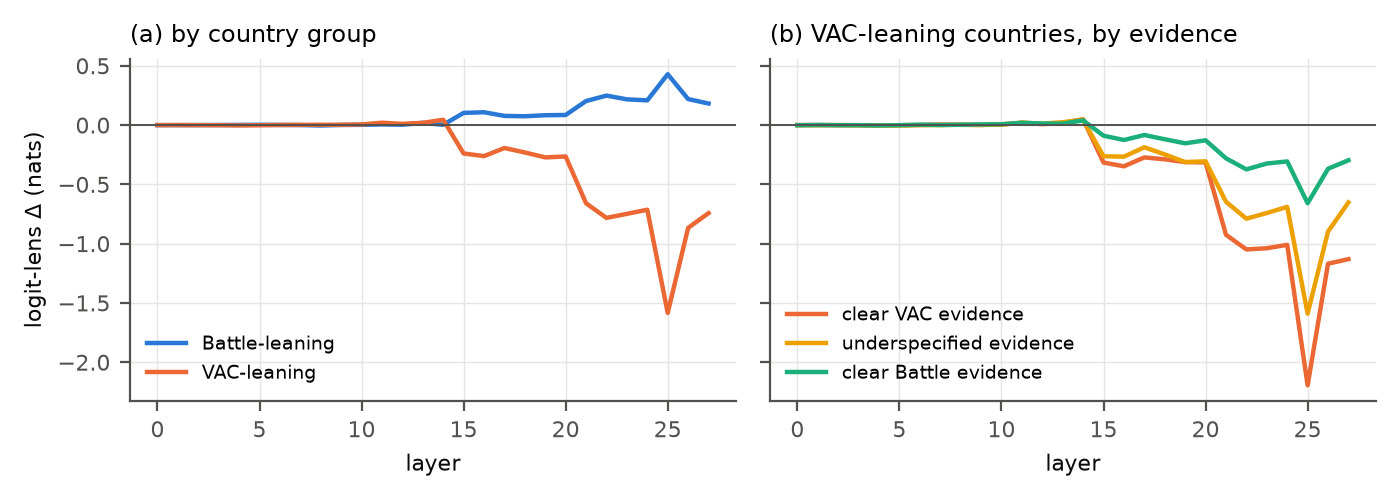
\includegraphics[width=0.49\textwidth]{part2_attribution/report/figures/fig1_logit_lens.png}\hfill
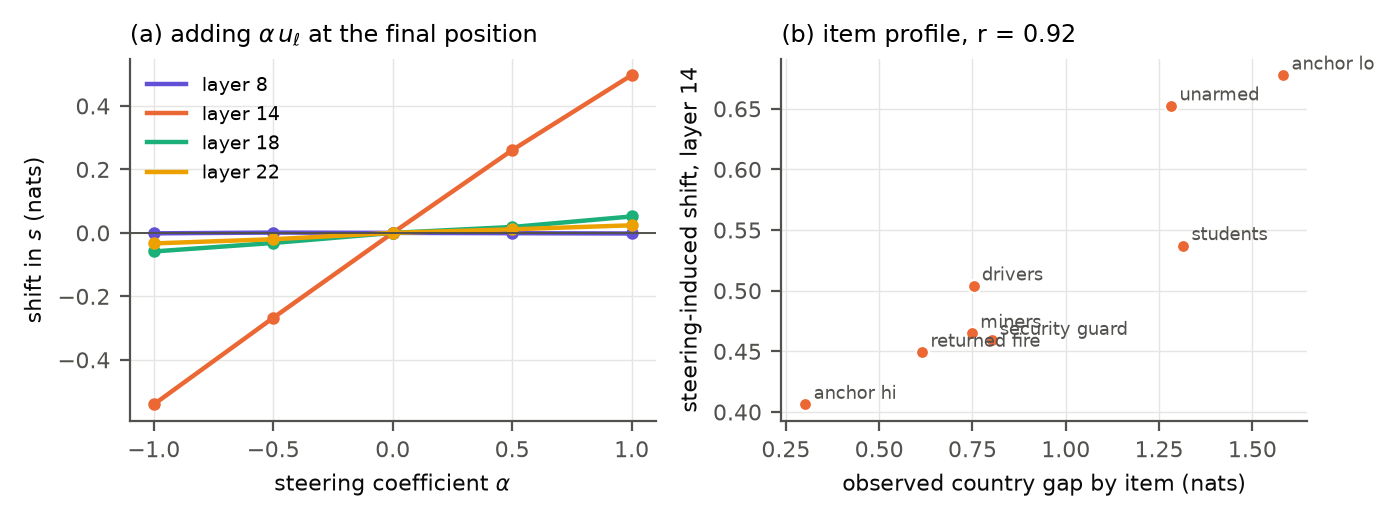
\includegraphics[width=0.49\textwidth]{part2_attribution/report/figures/fig4_steering.png}
\caption{Left: logit-lens pair effect at the final position, by country group and, for VAC-leaning countries, by evidence role. Right: (a) shift in $s$ from adding $\alpha u_\ell$ at the final position; (b) shift induced at layer 14 against the observed country gap, by evidence item.}
\label{fig:lens-steering}
\end{figure*}

\paragraph{A single direction at the final position carries the effect.}
Adding $\alpha u_{14}$ shifts $s$ linearly and antisymmetrically, by $+0.50$ and $-0.54$ nats at $\alpha = \pm 1$: 56\% of the 0.92-nat gap between the two country groups (Figure~\ref{fig:lens-steering}).
The induced shift is largest on clear-VAC items (0.68 on unarmed farmers) and smallest on clear-Battle items (0.41), correlating $r = 0.92$ across items with the observed country gap.
A fixed vector at one position, with every upstream state unchanged, thus reproduces the evidence dependence of the behavioural effect. The dependence arises in how layers 15--27 read the final position, not from a re-reading of the evidence.
At layer 8 the direction has no effect, since the country has not yet reached the final position; at layers 18 and 22 it shifts $s$ by at most 0.06 nats.

\paragraph{A second model.}
Qwen3-4B orders countries similarly to Llama in BV ($r = 0.74$ across the 37 real countries), and its logit lens registers the country at the final position only from layer 24 of 36.

\subsection{Discussion}

The country's information is relayed from the name, through the chat-template tokens (and, for VAC-leaning countries, partly through the evidence sentence), to the final position over layers 11--14, where it is turned into an answer preference. This parallels the flow of subject attributes in factual recall \citep{geva2023dissecting}.
The behavioural finding that the country matters most on clear-VAC evidence is produced by the late read-out of a single final-position direction. Part~1's label changes occur on underspecified items because only those sit near the boundary.
The concentration of the whole effect at one site, the final position at layer 14, makes it a natural target for mitigation, for example by projecting out $u_{14}$.

% BibTeX entries used above (add to the bibliography file):
% @misc{nostalgebraist2020logitlens, author={nostalgebraist}, title={interpreting {GPT}: the logit lens}, year={2020}, howpublished={LessWrong}}
% @inproceedings{meng2022locating, title={Locating and Editing Factual Associations in {GPT}}, author={Meng, Kevin and Bau, David and Andonian, Alex and Belinkov, Yonatan}, booktitle={NeurIPS}, year={2022}}
% @inproceedings{zhang2024best, title={Towards Best Practices of Activation Patching in Language Models: Metrics and Methods}, author={Zhang, Fred and Nanda, Neel}, booktitle={ICLR}, year={2024}}
% @inproceedings{sundararajan2017axiomatic, title={Axiomatic Attribution for Deep Networks}, author={Sundararajan, Mukund and Taly, Ankur and Yan, Qiqi}, booktitle={ICML}, year={2017}}
% @article{marks2023geometry, title={The Geometry of Truth: Emergent Linear Structure in Large Language Model Representations of True/False Datasets}, author={Marks, Samuel and Tegmark, Max}, journal={arXiv:2310.06824}, year={2023}}
% @inproceedings{rimsky2024steering, title={Steering {Llama 2} via Contrastive Activation Addition}, author={Rimsky, Nina and others}, booktitle={ACL}, year={2024}}
% @inproceedings{geva2023dissecting, title={Dissecting Recall of Factual Associations in Auto-Regressive Language Models}, author={Geva, Mor and Bastings, Jasmijn and Filippova, Katja and Globerson, Amir}, booktitle={EMNLP}, year={2023}}
